% *********************************************************************
% © 2021–2024 Jeremy Sylvestre
%
% Permission is granted to copy, distribute and/or modify this document
% under the terms of the GNU Free Documentation License, Version 1.3 or
% any later version published by the Free Software Foundation; with no
% Invariant Sections, no Front-Cover Texts, and no Back-Cover Texts. A
% copy of the license is included in the appendix entitled “GNU Free
% Documentation License” that appears in the output document of this
% PreTeXt source code. All trademarks™ are the registered® marks of
% their respective owners.
%
% *********************************************************************

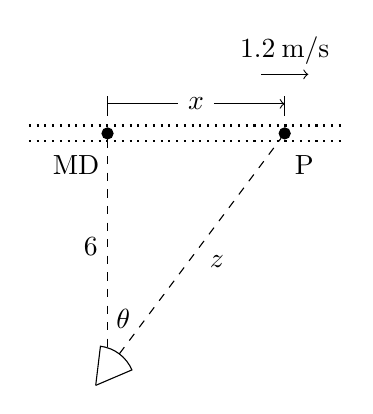
\begin{tikzpicture}
[
	closedpt/.style={circle,draw,fill,inner sep=0pt,minimum size=4pt},
	openpt/.style={circle,draw,inner sep=0pt,minimum size=4pt},
	scale=0.5
]

	\node[closedpt] at (0,6) (md) {};
	\node[xshift=-0.4cm,yshift=-0.4cm] at (0,6) {MD};
	\node[closedpt] at (4.5,6) (p) {};
	\node[xshift=0.25cm,yshift=-0.4cm] at (4.5,6) {P};

	\draw[thick,dotted] (-2,6.2) -- (6,6.2);
	\draw[thick,dotted] (-2,5.8) -- (6,5.8);

	\draw (0.3,0.4) arc (53:23:1cm) -- (-0.3,-0.4);
	\draw (0.3,0.4) arc (53:83:1cm) -- (-0.3,-0.4);
	\draw[dashed] (0.3,0.4) to node[below right] {$z$} (p);
	\draw[dashed] (md) to node[left] {$6$} (0,0.4);

	\node at (2.25,6.75) (x) {$x$};
	\draw[thin] (0,6.45) -- (0,6.95);
	\draw[thin] (4.5,6.45) -- (4.5,6.95);
	\draw[thin] (0,6.75) -- (x);
	\draw[thin,->] (x) -- (4.5,6.75);

	\draw[->] (3.9,7.5) -- node[above] {$1.2\:\mathrm{m}/\mathrm{s}$} (5.1,7.5);
	\node at (0.4,1.3) {$\theta$};

\end{tikzpicture}
